%!TEX root =../quadrotorbook.tex

\chapter{Camera Models and Feature Detection}
\label{chap:camera_features}

Figure~\ref{fig:image_pixels} shows a simple representation of a grayscale image.  The image is $M_x$ pixels wide, and $M_y$ pixels in height.  Image arrays are typically index from the top-left corner.  For example in \texttt{openCV} the $(0,0)$ pixel is the top-left pixel of the image, and the $(M_x, M_y)$ pixel is in the bottom right.  The center pixel will be denoted $(c_x, c_y)\approx (M_x/2, M_y/2)$. 
\begin{marginfigure}
  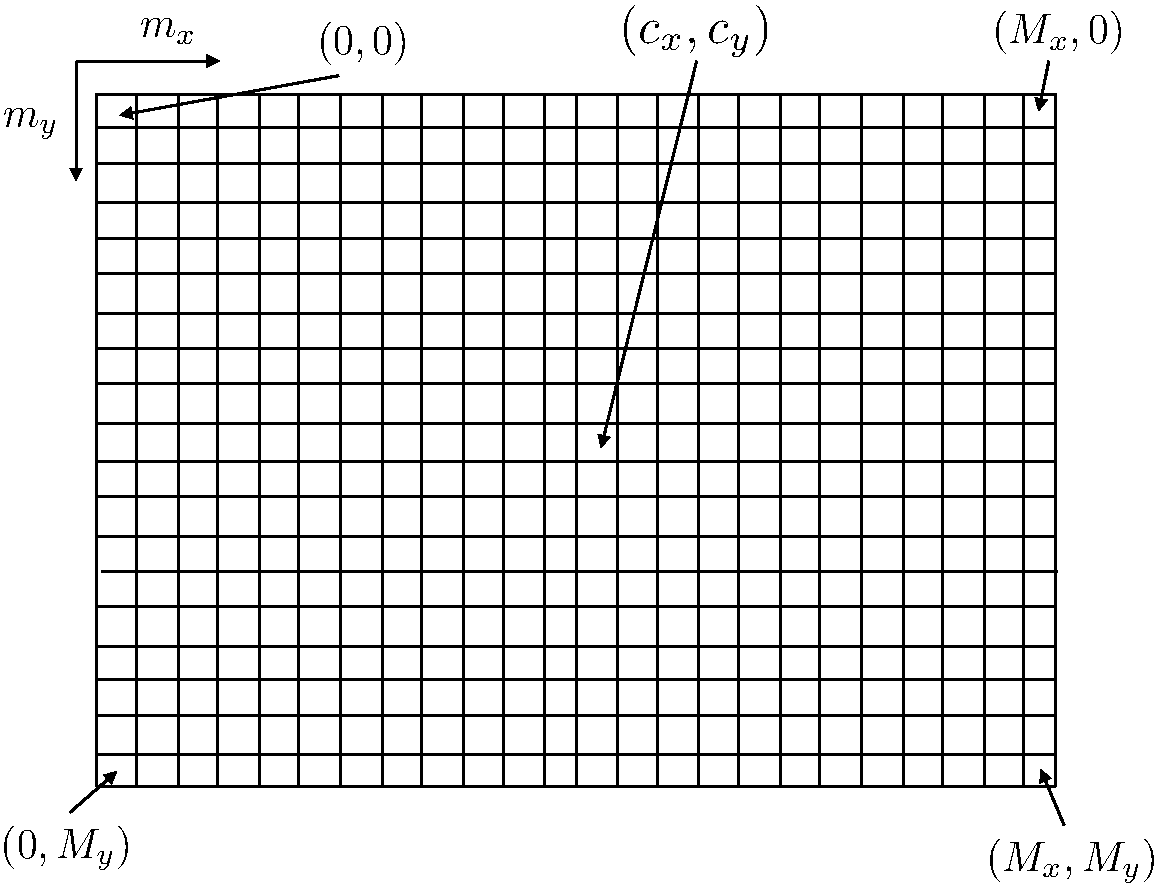
\includegraphics[width=\linewidth]{chap6_camera_features/figures/image_pixels}
  \caption{Image formation represented as pixels}
  \label{fig:image_pixels}  
\end{marginfigure}
The intensity of a grayscale image at pixel $(m_x, m_y)$ will be denoted $I(M_x,m_y)$ and is  typically represented as an integer value between $0$ (black) and $255$ (white).  
\marginnote{In this book we will work exclusively with grayscale images.  Most cameras return color image, which consists of three $M_x\times M_y$ arrays representing, for example B(blue), G(green), R(red).  In \texttt{openCV} BGR images can be converted to grayscale using the command \texttt{grayimage=cv2.cvtColor(colorimage, cv2.COLOR\_BGR2GRAY)}.}


%------------------------------------------------------------
\section{Pinhole model}
\label{sec:pin_hole_model}

The geometry of camera is shown in Figure~\ref{fig:pin_hole_camera}.
The camera frame is represented as $\mathcal{F}_c = \{\ibf_c, \jbf_c, \kbf_c\}$, where $\ibf_c$ is aligned with the $m_x$-direction in the image plane, i.e., to the right when looking at the image, $\ibf_y$ is aligned with $m_y$-direction in the image plane, i.e., down when looking at the image, and $\kbf_c$ is aligned along the optical axis, or in the pointing direction of the camera, and so that a scaled version of $\kbf_c$ would intersect the image plane at the center of the image.  The image plane is located at a distance $Sf$ from the center of the camera frame, where $f$ is the focal length in units of pixels, and $S$ is a scale factor that converts pixels to meters.  
\begin{figure}[htb]
  \label{fig:pin_hole_camera}
  \centering
  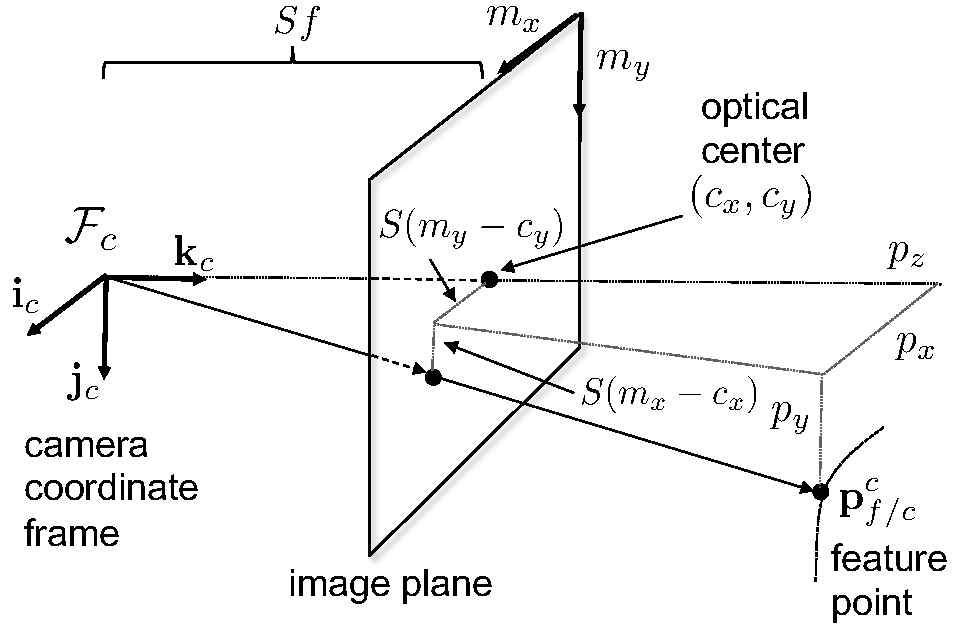
\includegraphics[width=\linewidth]{chap6_camera_features/figures/pin_hole_camera}
  \caption{Pin hole camera model}
\end{figure}

Let $\pbf_{f/c}^c = (p_x, p_y, p_z)^\top$ be the 3D Euclidian position of a feature point in the environment relative to the camera frame, expressed in the camera frame, as shown in Figure~\ref{fig:pin_hole_camera}.  Suppose that the projection of the point $\pbf_{f/c}^c$ on to the camera frame is at  the pixel $(m_x, m_y)$.  The vector that represents the projection of $\pbf_{f/c}^c$ on the image plane is given by
\[
\begin{pmatrix} S(m_x-c_x) \\ S(m_y-c_y) \\ Sf \end{pmatrix}.
\]

From Figure~\ref{fig:pin_hole_camera} and using similar triangles, we get that
\begin{align*}
\frac{S(m_x-c_x)}{Sf} &= \frac{p_x}{p_z} \\	
\frac{S(m_y-c_y)}{Sf} &= \frac{p_y}{p_z},
\end{align*}
or equivalently
\begin{align*}
m_x &= c_x + f\frac{p_x}{p_z} \\	
m_y &= c_y + f\frac{p_y}{p_z}.
\end{align*}
In order to write the pixel location as vector, we introduce {\em normalized homogeneous coordinates} to write
\begin{align}
\begin{pmatrix}m_x \\ m_y \\ 1\end{pmatrix} 
	&= \begin{pmatrix} c_x(p_z/p_z) + f\frac{p_x}{p_z} \\ c_y(p_z/p_z) + f\frac{p_y}{p_z} \\ (p_z/p_z) \end{pmatrix} \notag \\
	&= \frac{1}{p_z}\begin{pmatrix} f & 0 & c_x \\ 0 & f & c_y \\ 0 & 0 & 1 \end{pmatrix}\begin{pmatrix}p_x \\ p_y \\ p_z \end{pmatrix}.
	\label{eq:intrinsic_parameters_1}
\end{align}
%
For real-world cameras, the focal length can be different in the $x$ and $y$ directions.  Consider Figure~\ref{fig:focal_length_calculation}.
\begin{marginfigure}
  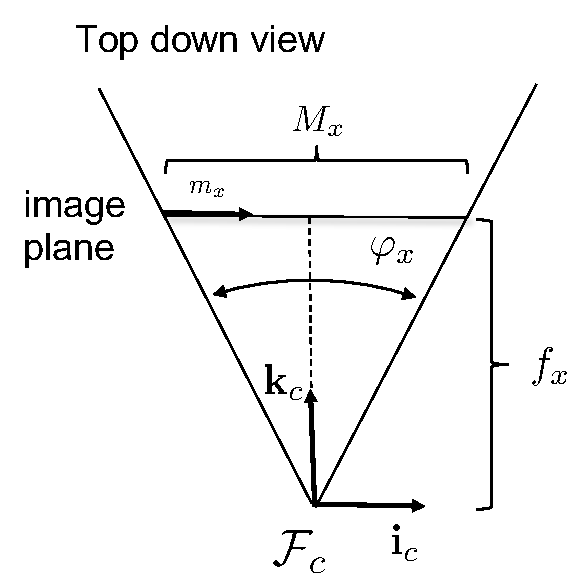
\includegraphics[width=\linewidth]{chap6_camera_features/figures/focal_length_calc}
  \caption{Calculation of the focal length in the image $x$-direction.}
  \label{fig:focal_length_calculation}  
\end{marginfigure}
Suppose that the camera field of view in the $x$ direction is $\varphi_x$, and that the size of image array in the $x$-direction is $M_x$.  Then we have 
\begin{align*}
& \tan\left(\frac{\varphi_x}{2}\right) = \frac{(M_x/2)}{f_x} \\
\implies & f_x = \frac{M_x}{2\tan\left(\frac{\varphi_x}{2}\right)}.
\end{align*}
Therefore Equation~\eqref{eq:intrinsic_parameters_1} becomes
\[
\begin{pmatrix}m_x \\ m_y \\ 1\end{pmatrix} 
	= \frac{1}{p_z}\begin{pmatrix} f_x & 0 & c_x \\ 0 & f_y & c_y \\ 0 & 0 & 1 \end{pmatrix}\begin{pmatrix}p_x \\ p_y \\ p_z \end{pmatrix}.
\]
It turns out that for real cameras, not only are the pixels not square, but they can also be skewed.  The skew factor can be represented by\cite{MaSoattoKoseckaSastry03}
\[
\begin{pmatrix}m_x \\ m_y \\ 1\end{pmatrix} 
	= \frac{1}{p_z}\begin{pmatrix} f_x & f_\theta & c_x \\ 0 & f_y & c_y \\ 0 & 0 & 1 \end{pmatrix}\begin{pmatrix}p_x \\ p_y \\ p_z \end{pmatrix}.
\]
where $f_\theta$ is also in units of pixels.  
Defining 
\[
K_c \doteq \begin{pmatrix}f_x & f_\theta & c_x \\ 0 & f_y & c_y \\ 0 & 0 & 1\end{pmatrix}
\]
to be the intrinsic parameters of the camera, we have shown that 
\begin{equation}\label{eq:pin_hole_pixel}
\lambda_f \begin{pmatrix} m_x \\ m_y \\ 1 \end{pmatrix} = K_c \pbf_{f/c}^c,
\end{equation}
where $\lambda_f = p_z$ is the (unknown) distance to the feature along the camera $z$-axis.  
\marginnote{In \texttt{ROSflight-Holodeck}, the horizontal field-of-view of the camera is $90$ degrees from which $f_x$ can be computed.  Assume that $f_y=f_x$ and $f_\theta=0$.  The optical center can be computed as $c_\ast = M_\ast/2$.}

The intrinsic parameters $K_c$ (in addition to radial distortion parameters) can be found through a process known as camera calibration.  If the camera has been calibrated, then $K_c$ is known.  When $K_c$ is known, then pixel coordinated returned via $\texttt{openCV}$ can be converted to calibrated pixel coordinates as 
\begin{equation}\label{eq:calibrated_normalized_homogeneous_coord}
\begin{pmatrix} \epsilon_x \\ \epsilon_y \\ 1 \end{pmatrix} = K_c^{-1} \begin{pmatrix} m_x \\ m_y \\ 1 \end{pmatrix},
\end{equation}
where we have the simplified formula
\sidenote{Note that in this formula $\epsilon_x$ and $\epsilon_y$ are unitless since $K_c$, $m_x$, and $m_y$ have units of pixels.}
\[
\lambda_f \bar{\epsilonbf}_{f/c}^c = \pbf_{f/c}^c.
\]

If pixel coordinates are in the form $\mbf = (m_x, m_y, m_z)^\top$ where $m_z$ is arbitrary, then we say that the pixel is represented in {\em homogeneous coordinates}.  If the last element is equal to one, then we say that the pixel is in {\em normalized homogeneous coordinates}. If the pixel coordinates have been calibrated as in Equation~\eqref{eq:calibrated_normalized_homogeneous_coord}, then we say that the pixel is in {\em calibratated normalized homogeneous coordinates}.
%
Unless otherwise stated, we will assume pixel coordinates are represented using calibrated normalized homogeneous coordinates.

Recall from Section~\ref{sec:homogeneous transformations} that position vectors can be presented in homogeneous coordinates by appending a $1$ as the fourth element.  In homogeneous coordinates we have\cite{MaSoattoKoseckaSastry03}
\[
\lambda_f \bar{\epsilonbf}_{f/c}^c = \Pi_0\bar{\pbf}_{f/c}^c,
\]
where
\[
\Pi_0 \doteq \begin{pmatrix} 1 & 0 & 0 & 0 \\ 0 & 1 & 0 & 0 \\ 0 & 0 & 1 & 0 \end{pmatrix}.
\]
Recall also from Section~\ref{sec:homogeneous transformations} that the position of the feature in the camera frame, can be related to the position of the feature in the inertial frame via the homogeneous transformation
\[
\bar{\pbf}_{f/c}^c = T_i^c \bar{\pbf}_{f/i}^i = \begin{pmatrix} R_i^c & \tbf_{i/c}^c \\ 0 & 1 \end{pmatrix} \bar{\pbf}_{f/i}^i.
\]
Therefore, the calibrated camera model becomes
\begin{equation}\label{eq:pin_hole_calibrated}
\lambda_f \bar{\epsilonbf}_{f/c}^c = \Pi_0 T_i^c \bar{\pbf}_{f/i}^i.
\end{equation}

%------------------------------------------------------------
\section{Camera Field of View}
\label{sec:field_of_view}

Figure~\ref{fig:field_of_view} shows the field of view of a pin-hole camera.  
\begin{figure}
  \centering
  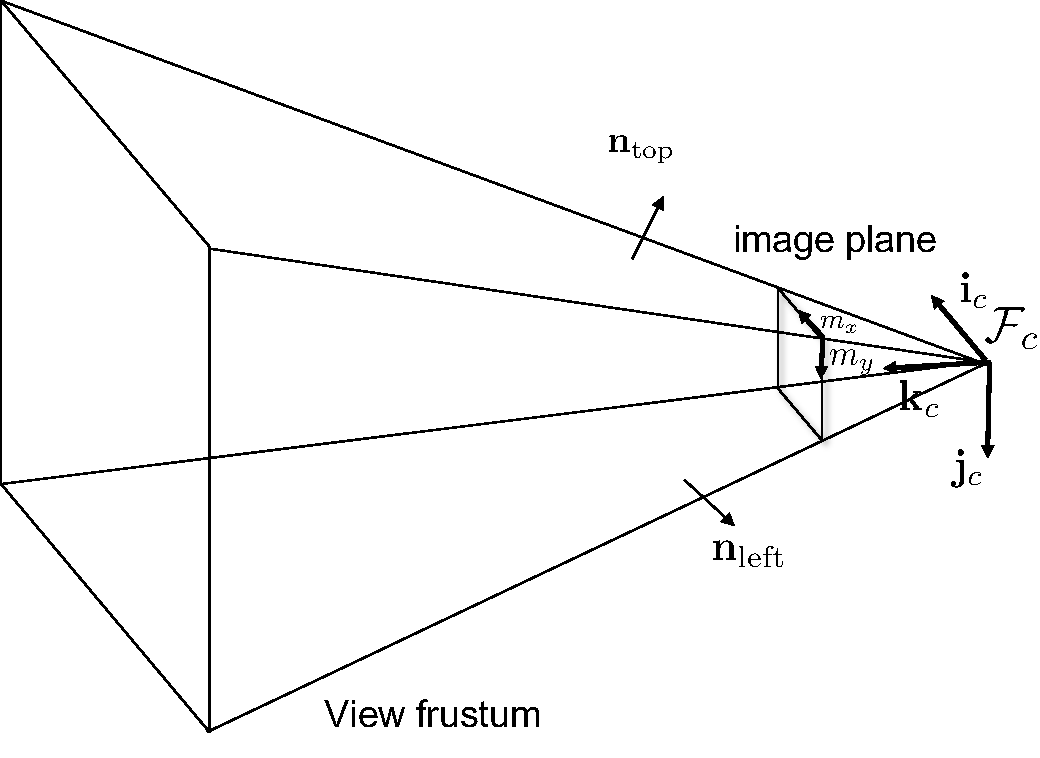
\includegraphics[width=0.8\textwidth]{chap6_camera_features/figures/field_of_view}
  \caption{The field of view of a pin-hole camera is a pyramidal frustum.}
  \label{fig:field_of_view}
\end{figure}
The view frustum originates at the origin of the camera coordinate frame $\mathcal{F}_c$.  The field of view can be represented as the intersection of four half planes in $\mathbb{R}^3$.  The half planes are described by the equations
\begin{align*}
\mathbf{n}_{\text{right}}^{i\top}(\mathbf{r}-\mathbf{p}_{c/i}^i) &\leq 0 \\
\mathbf{n}_{\text{left}}^{i\top}(\mathbf{r}-\mathbf{p}_{c/i}^i) &\leq 0 \\
\mathbf{n}_{\text{top}}^{i\top}(\mathbf{r}-\mathbf{p}_{c/i}^i) &\leq 0 \\
\mathbf{n}_{\text{bottom}}^{i\top}(\mathbf{r}-\mathbf{p}_{c/i}^i) &\leq 0 
\end{align*}
where $\mathbf{p}_{c/i}^i$ is the position of the origin of the camera frame with respect to the inertial frame, expressed in the inertial frame, and $\mathbf{n}_{\ast}^i$ are unit vectors that are perpendicular to the sides of the view frustum, expressed in the inertial frame.  

Since the unit vectors $\mathbf{n}_{\ast}$ are fixed in the camera frame, we can write
\[
\mathbf{n}_{\ast}^i = R_c^i \mathbf{n}_{\ast}^c.
\]
%
Defining the matrix
\[
N = \begin{pmatrix} \mathbf{n}_{\text{right}}^c & \mathbf{n}_{\text{left}}^c & \mathbf{n}_{\text{top}}^c & \mathbf{n}_{\text{bottom}}^c \end{pmatrix},
\]
then the view frustum $\mathcal{F}$ is given by
\[
\mathcal{F}(\mathbf{p}_{c/i}^i, R_c^i) = \{\mathbf{r}\in\mathbb{R}^3: N^\top (R_c^i)^\top  (\mathbf{r}-\mathbf{p}_{c/i}^i)\leq \mathbf{0} \}.
\]

To find the unit vectors $\mathbf{n}_{\ast}$, consider the top down view of the camera field of view shown in Figure~\ref{fig:field_of_view_top_down}.  
\begin{marginfigure}
  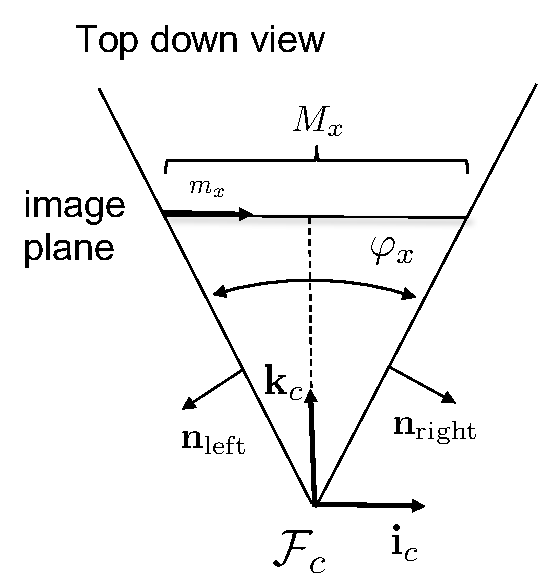
\includegraphics[width=\linewidth]{chap6_camera_features/figures/fov_calc}
  \caption{A top down view of the field of view.}
  \label{fig:fov_calc}
\end{marginfigure}
Let $M_x$ be the number of pixels along the camera $x$-direction, and let $f$ be the focal length given in pixels.  Then the angular arc defining the field of view in the $x$-direction is given by
\[
\varphi_x = 2\tan^{-1}\left(\frac{M_x}{2f}\right).
\]
Accordingly, from geometry we have 
\begin{align*}
\mathbf{n}_{\text{right}} &= \left(\cos\left(\frac{\varphi_x}{2}\right), 0, -\sin\left(\frac{\varphi_x}{2}\right) \right)^\top \\
\mathbf{n}_{\text{left}} &= \left(-\cos\left(\frac{\varphi_x}{2}\right), 0, -\sin\left(\frac{\varphi_x}{2}\right) \right)^\top.
\end{align*}
Similar arguments give
\begin{align*}
\mathbf{n}_{\text{top}} &= \left(0, -\cos\left(\frac{\varphi_y}{2}\right), -\sin\left(\frac{\varphi_x}{2}\right) \right)^\top \\
\mathbf{n}_{\text{bottom}} &= \left(0, \cos\left(\frac{\varphi_y}{2}\right), -\sin\left(\frac{\varphi_y}{2}\right) \right)^\top,
\end{align*}
where
\[
\varphi_y = 2\tan^{-1}\left(\frac{M_y}{2f}\right),
\]
and $M_y$ is the number of pixels in the camera $y$-direction.

\begin{lemma}
	If the size of the pixel array is given by $M_x \times M_y$, and the camera calibration matrix is given by
	\[
	K_c = \begin{pmatrix} f_x & 0 & c_x \\ 0 & f_y & c_y \\ 0 & 0 & 1 \end{pmatrix}
	\]
	then the normalized homogeneous coordinates
	\[
	\epsilonbf = (\epsilon_x, \epsilon_y, 1)^\top
	\]
	 are in the camera field of view if and only if
	\begin{align*}
	-\frac{c_x}{f_x} \leq &\epsilon_x \leq \frac{M_x - c_x}{f_x} \\
	-\frac{c_y}{f_y} \leq &\epsilon_y \leq \frac{M_y - c_y}{f_y}.
	\end{align*}
\end{lemma}
\begin{proof}
	The pixel $m_\ast$ is in the field of view if and only if
	\[
	0 \leq m_\ast \leq M_\ast.
	\]
	The result follow from simple manipulation using the fact that
	$m_\ast = f_\ast \epsilon_\ast + c_\ast$.
\end{proof}


%------------------------------------------------------------
\section{Some notes on Points and lines in images}
See~\cite{MaSoattoKoseckaSastry03} 

A point in an image is actually a line in 3D space.  Figure~\ref{fig:point_and_line} shows a normalized pixel $\epsilonbf$ 
in the image plane.  Note that in fact the point $\epsilonbf$ defines a line (or linear space) in $\mathbb{R}^3$ given by $k\epsilonbf$ that originates at the origin of $\mathcal{F}_c$ and passes through $\epsilonbf$.  We say that two points given in homogenous coordinates are equivalent if they are equal up to a scale factor, i.e., we write $\xbf = \ybf$ if $\xbf = \lambda \ybf$ for some $\lambda$.  

Define the two dimensional projective space $\mathbb{P}^2$ to be the set of all homogeneous coordinates.\cite{HartleyZisserman03}  Therefore if $\xbf, \ybf \in \mathbb{P}^2$, then $\xbf=\ybf$ if $\xbf = \lambda \ybf$ for some $\lambda\in\mathbb{R}$.  
Note that if $\xbf=\ybf$, then their vector components will be equal if they are placed in normalized homogeneous coordinates.  
\begin{figure}
	\centering
	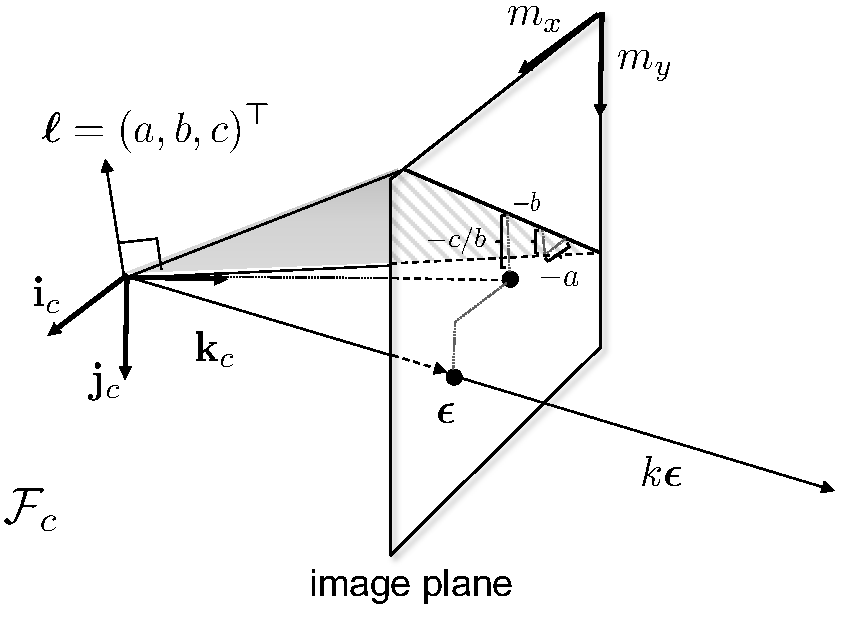
\includegraphics[width=0.8\textwidth]{chap6_camera_features/figures/point_and_line}
	\caption{A point $\epsilonbf$ in the image is a linear space in $\mathbb{R}^3$, and a line $\ellbf$ is the image.}
	\label{fig:point_and_line}
\end{figure}

The equation for a line in the image plane is given by
\[
\epsilon_y = m\epsilon_x + b,
\]
where $m$ is the slope and $b$ is the intercept with the $y$-axis.  More generally, a line in the image plane is given by
\[
a \epsilon_x + b\epsilon_y + c = 0,
\]
thee the slope is $-a/b$ and the $y$-intercept is $-c/b$.  The line is depicted graphically in Figure~\ref{fig:point_and_line}.  Let $\ellbf \defeq (a, b, c)^\top$ and note that $\epsilonbf$ is on the line $\ellbf$ if and only if
\[
\ellbf^\top \epsilonbf = 0.
\]
In 3D space, the line $\ellbf$ in the image plane is the projection of a 2D plane in 3D that passes through the origin of $\mathcal{F}_c$ and intersects the image plane at the line.  The 3D vector $\ellbf$ is normal to this plane.  For example, the line along the image $x$-axis is given by $\epsilon_y=0$, and the corresponding line is 
\[
0\epsilon_x + 1 \epsilon_y + 0 = \begin{pmatrix}0 \\ 1 \\ 0\end{pmatrix}^\top \begin{pmatrix}\epsilon_x \\ \epsilon_y \\ 1 \end{pmatrix}=0.
\]
The line $\ellbf=(0, 1, 0)^\top$ is perpendicular to the plane that intersects the image plane along the $x$-axis.  Since the scaling of $\ellbf$ doesn't change the fact that it is parallel to the corresponding plane, we see that $\ellbf \in \mathbb{P}^2$ defines a line in the image (i.e., for any scale).  Therefore, both lines and points can be represented by homogenous coordinates.  

Suppose that there are two lines in the image given by $\ellbf_1, \ellbf_2\in\mathbb{P}^2$, then if the lines are not parallel, the associated planes will intersect at a line given by $\ellbf_1 \times \ellbf_2$ which corresponds to the image point $\epsilonbf = \ellbf_1\times\ellbf_2$, where $\epsilonbf\in\mathbb{P}^2$ is given in homogeneous coordinates.  If the lines are parallel, then their slopes are equal, but the $y$-intercept may be different.  Therefore, parallel lines will have the form
\[
\ellbf_1 = \begin{pmatrix} a \\ b \\ c_1 \end{pmatrix}, \qquad \qquad \ellbf_2 = \begin{pmatrix} ka \\ kb \\ kc_2 \end{pmatrix},
\]
and the cross product is given by
\[
\ellbf_1 \times \ellbf_2 =  \begin{pmatrix} kb (c_2-c_1) \\ ka(c_1-c_2) \\ 0 \end{pmatrix}.
\]
Therefore, in homogeneous coordinates, a zero in the third element represents point at infinity.~\cite{HartleyZisserman03}

Given two image points represented in homogeneous coordinates $\epsilonbf_1, \epsilonbf_2\in\mathbb{P}^2$, the line in the image that contains both of these points will be defined by a plane that contains both rays.  A perpendicular vector to that plane is therefore given by
\[
\ellbf = \epsilonbf_1 \times \epsilonbf_2 \in \mathbb{P}^2.
\]

We have therefore shown the following theorem.
\begin{theorem}
	Let $\epsilonbf_1, \epsilonbf_2\in\mathbb{P}^2$ represent two points in the image plane, and let $\ellbf_1, \ellbf_2\in\mathbb{P}^2$ represent two lines in the image plane.  Then
	\begin{enumerate}
		\item The point $\epsilonbf_1$ is on the line $\ellbf_1$ if and only iff $\epsilonbf_1^\top \ellbf_1 = 0$.
		\item The line that contains both $\epsilonbf_1$ and $\epsilonbf_2$ is given in homoogeneous coordinates as $\ellbf = \epsilonbf_1 \times \epsilonbf_2$.
		\item The lines $\ellbf_1$ and $\ellbf_2$ intersect at the point given in homogeneous coordinates as $\epsilonbf = \ellbf_1 \times \ellbf_2$.
	\end{enumerate} 
\end{theorem}


%------------------------------------------------------------
\section{Feature Detection}
\label{sec:feature_detection}

\rwbcomment{Need to add some images with features to this section.}

The image based control and estimation schemes that we will consider in this book will primarily be based on feature detection and feature tracking.  In this section we discuss the Harris corner detector and the related Shi-Tomasi corner detector. 
\marginnote{The \texttt{openCV} function \texttt{goodfeaturestotrack} uses the Shi-Tomasi algorithm to find good features to track.}
%
\marginnote{A nice overview of Features and the Shi-Tomasi feature detector is given at \url{https://aishack.in/tutorials/features}.}
	
The Harris corner detector attempts to find positions in the image that have strong gradients in both the $x$ and $y$ directions. Consider the function
\[
E_{\mathbf{m}}'(u,v) = \abs{I(m_x + u, m_y+v) - I(m_x, m_y)}^2
\]
which is a function of pixel deviations $(u,v)$.  For example, if $E_{\mathbf{m}}'(1,0)$ is large, then the image intensity undergoes a large change for one pixel deviation along the $x$-direction in the image.  
It is desireable to find features that are well-defined over a window $W$ of pixels.  For example, noise may cause strong gradients at one pixel in the image, but the gradient in each direction does not persist for more than a few pixels.  Define the window $W(\mbf)$ to be an $(N+1)\times(N+1)$ box around the pixel $\mbf$.  Consider the cost function
\[
E_{\mathbf{m}}(u,v) = \sum_{(x,y)\in W(\mbf)} \abs{ I(x+u, y+v)-I(x,y) }^2,
\]
then good features will be those pixels $\mbf$ where $E$ is large.
Using the Taylor series approximation of image intensity $I(x,y)$ we get
\begin{equation}\label{eq:image_gradient_1}
I(x+u, y+v) = I(x,y) + \frac{\partial I}{\partial x}(x,y)u + \frac{\partial I}{\partial y}(x,u) v + H.O.T.
\end{equation}

Given an image $I(x, y)$, the gradient image along the $x$-direction can be found by convolving the image with the so-called Sobel edge detector
\[
G_x = \left[ \begin{array}{c|c|c}
-1 & 0 & 1 \\\hline -2 & 0 & 2 \\\hline -1 & 0 & 1
\end{array} \right]
\]

Similarly, the gradient along the $y$-direction can be found by convolving the image with
\[
G_y = \left[\begin{array}{c|c|c}
-1 & -2 & -1  \\\hline 0 & 0 & 0  \\\hline 1 & 2 & 1
\end{array} \right].
\]
Equivalently, the gradient $\frac{\partial I}{\partial \mbf}$ of an image at pixel $\mbf^0=(m_x^0, m_y^0)^\top$ is given by
\begin{equation}\label{eq:image_gradient}
\frac{\partial I}{\partial \mbf}(\mbf^0) \defeq
\begin{pmatrix} I_x \\ I_y \end{pmatrix}
= \left(\begin{array}{c}
[I(m_x^0+1, m_y^0-1)-I(m_x^0-1,m_y^0-1)] \\
+ 2[I(m_x^0+1, m_y^0)-I(m_x^0-1,m_y^0)] \\
+ [I(m_x^0+1, m_y^0+1)-I(m_x^0-1,m_y^0+1)] \\\hline
 [I(m_x^0-1, m_y^0+1)-I(m_x^0-1,m_y^0-1)] \\
+ 2[I(m_x^0, m_y^0+1)-I(m_x^0,m_y^0-1)] \\
+ [I(m_x^0+1, m_y^0+1)-I(m_x^0+1,m_y^0-1)]
\end{array}\right).
\end{equation}

Therefore, dropping all be the constant and linear terms in Equation~\eqref{eq:image_gradient_1} gives
\begin{align*}
E_{\mathbf{m}}(u,v) &\approx \sum_{(x,y)\in W(\mbf)} \abs{I_x(x,y)u +I_y(x,y) v }^2,\\
&= \sum_{(x,y)\in W(\mbf)} \begin{pmatrix} u & v \end{pmatrix}\begin{pmatrix}\left(I_x(x,y)\right)^2 & I_x(x,y) I_y(x,y) \\
I_x(x,y)I_y(x,y) & (I_y(x,y))^2 \end{pmatrix}\begin{pmatrix}u \\ v\end{pmatrix} \\
&= \begin{pmatrix} u & v \end{pmatrix} G(\mbf) \begin{pmatrix}u \\ v\end{pmatrix},
\end{align*}
where
\begin{equation}\label{eq:G_mbf}
G(\mbf) = \sum_{(x,y)\in W(\mbf)} \begin{pmatrix}\left(I_x(x,y)\right)^2 & I_x(x,y) I_y(x,y) \\
I_x(x,y)I_y(x,y) & (I_y(x,y))^2 \end{pmatrix}.
\end{equation}
We are therefore interested in pixels $\mbf$ where $\xbf^\top G(\mbf) \xbf$ is large, where $\xbf\in\mathbb{R}^2$ is a unit vector.  Since $G(\mbf)$ is symmetric, its eigen-decomposition is given by
\[
G = U\begin{pmatrix} \lambda_1 & 0 \\ 0 & \lambda_2 \end{pmatrix} U^\top,
\] 
where $U$ is orthogonal.  Therefore $\xbf^\top G(\mbf) \xbf$ is large for all $\xbf$ when both of the eigenvalues of $G(\mbf)$ are large.  

\subsection{Harris Corner Detector}
The so-called Harris corner detector, originally proposed by (Harris \& Stephens)\cite{HarrisStephen88} uses the metric
\[
R_h = \det{G} - k~\trace{G}
\]
to distinguish good features.  
Since for any matrix
\begin{align*}
\det{A} &= \Pi \lambda_i \\
\trace{A} &= \sum \lambda_i,
\end{align*}
it follows that 
\[
R(G) = \lambda_1\lambda_2 - k(\lambda_1+\lambda_2),
\]
where $k$ is typically small.  Therefore $R$ will be large when both $\lambda_1$ and $\lambda_2$ are relatively large and close to the same size.

\subsection{Shi-Tomasi Corner Detector}
The Shi-Tomasi corner detector, originally proposed in (Shi \& Tomasi)~\cite{ShiTomasi94} instead uses the metric
\[
R_{st}(G) = \min\{\lambda_1, \lambda_2\}
\]
to distinguish good features.  In this case, $R(G)$ will be above a threshold when both eigenvalues are above that threshold.  The eigenvalues of $G$ can be found explicitly as 
\begin{align*}
\lambda_1 &= \frac{1}{2}\left(\sum_W I_x^2 + \sum_W I_y^2\right) + \frac{1}{2}\sqrt{(\sum_W I_x^2 - \sum_W I_y^2)^2+4(\sum_W I_x)^2(\sum_W I_y)^2}\\
\lambda_2 &=\frac{1}{2}\left(\sum_W I_x^2 + \sum_W I_y^2\right) - \frac{1}{2}\sqrt{(\sum_W I_x^2 - \sum_W I_y^2)^2+4(\sum_W I_x)^2(\sum_W I_y)^2},
\end{align*}
which implies that
\[
R_{st}(G(\mbf)) = \frac{1}{2}\left(\sum_W I_x^2 + \sum_W I_y^2\right) - \frac{1}{2}\sqrt{(\sum_W I_x^2 - \sum_W I_y^2)^2+4(\sum_W I_x)^2(\sum_W I_y)^2}.
\]



Python code for finding good features to track is shown here~
\sidenote{\href{https://docs.opencv.org/master/d4/d8c/tutorial_py_shi_tomasi.html}{OpenCV function}}

%
%\begin{lstlisting}[language=Python]
%import numpy as np
%import cv2 as cv
%from matplotlib import pyplot as plt
%from matplotlib import pyplot as plt
%img = cv.imread('image.jpg')
%gray = cv.cvtColor(img,cv.COLOR_BGR2GRAY)
%corners = cv.goodFeaturesToTrack(gray,25,0.01,10)
%corners = np.int0(corners)
%for i in corners:
%x,y = i.ravel()
%cv.circle(img,(x,y),3,255,-1)
%plt.imshow(img),plt.show()
%\end{lstlistng}

















